\subsubsection{Mockups}
Für die Erstellung der \Gls{Mockup}s wird das Tool Figma verwendet. Innerhalb eines geteilten Workspace werden erste Entwürfe für die fünf verschiedenen Menüs der Applikation erstellt. Damit wird gezeigt, welche Funktionen die App haben wird und wie das Design aussehen könnte.

\bigskip


\paragraph{Map}Der \Gls{Tab} „Map“ dient zur Darstellung der verfügbaren Möglichkeiten zur Lagerung von Fahrrädern in der Umgebung auf einer Karte. Mit einem Marker wird ein Fahrradturm dargestellt. Außerdem soll die Verfügbarkeit von freien Plätzen dargestellt werden.

\begin{figure}[H]
  \centering
  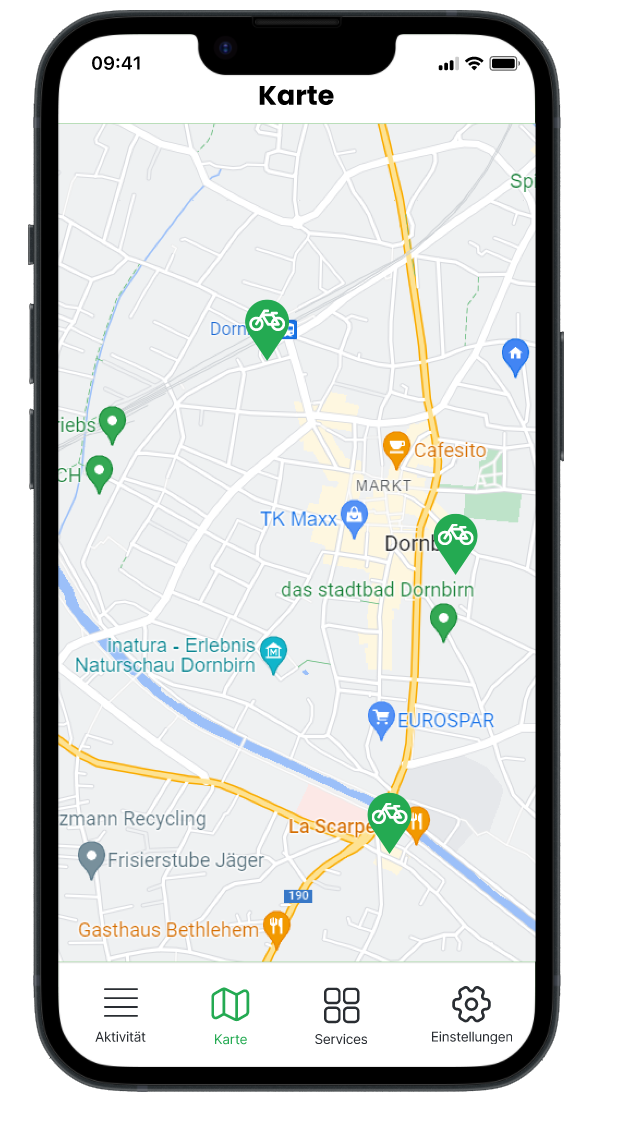
\includegraphics[width=0.3\textwidth]{images/app_mock_map}
  \caption{\Gls{Mockup} vom Screen Map}
  \label{fig:screenmapmock}
\end{figure}

\bigskip


\paragraph{Tower}Der \Gls{Tab} „Tower“ dient zur Anzeige folgender Informationen:

\begin{itemize}
  \item Karte mit Standort des Turmes
  \item Anzahl verfügbaren Lagerungsmöglichkeiten
  \item Bereits von der anwendenden Person bei diesem Turm gelagerte Gegenstände
  \item Möglichkeit zum Einlagern von einem weiteren Rad oder Gegenstand
\end{itemize}

\begin{figure}[H]
  \centering
  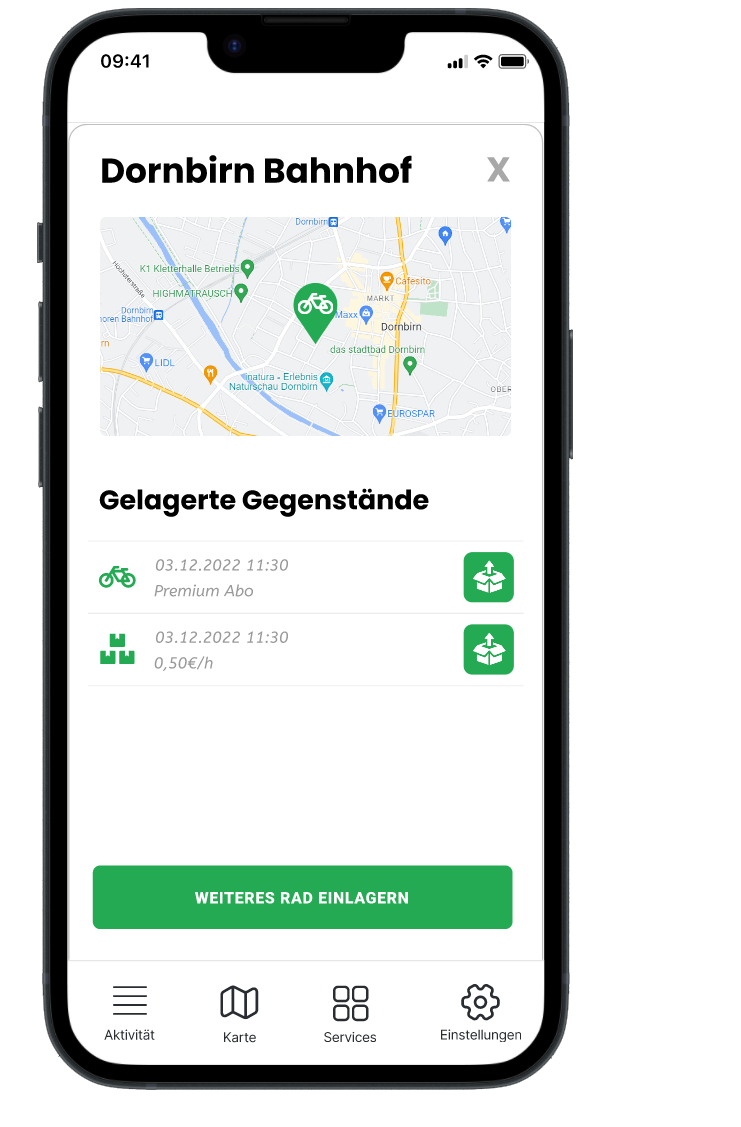
\includegraphics[width=0.3\textwidth]{images/app_mock_tower}
  \caption{\Gls{Mockup} vom Screen Tower}
  \label{fig:screentowermock}
\end{figure}

\bigskip


\paragraph{Aktivität}Im oberen Teil vom \Gls{Tab} „Aktivität“ werden die von der anwendenden Person gelagerten Gegenstände angezeigt. Auf der unteren Hälfte werden vergangene Buchungen mit weiteren Informationen aufgelistet. Falls man auf eine Buchung klickt, sollen weitere Infos erscheinen.

\begin{figure}[H]
  \centering
  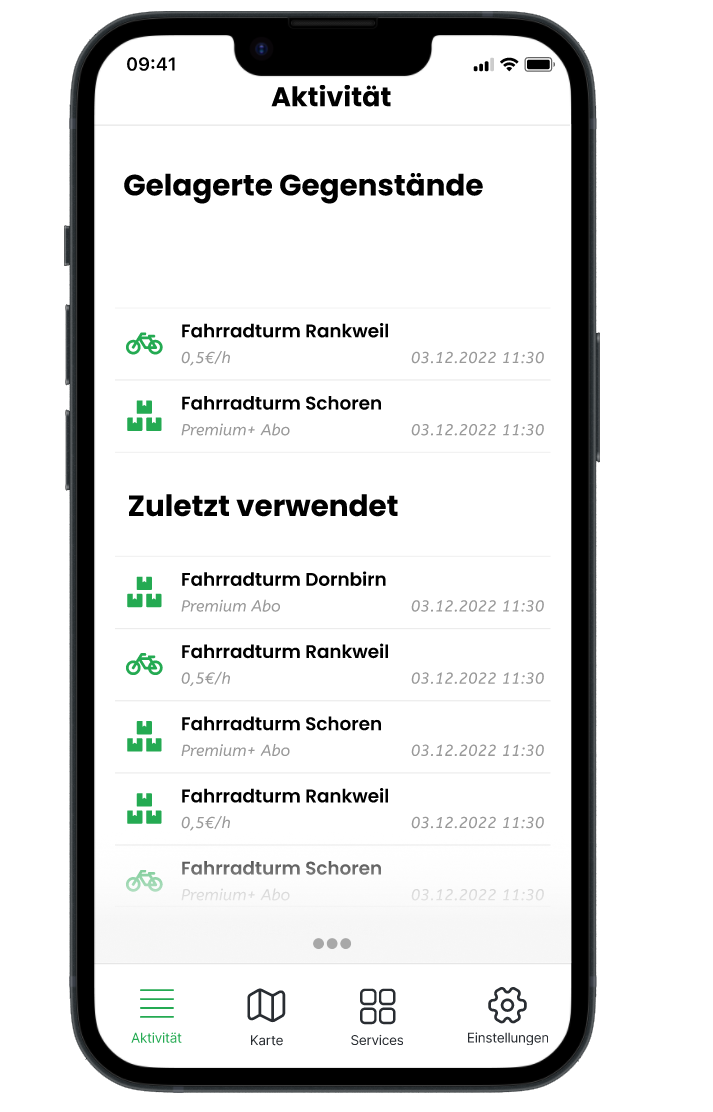
\includegraphics[width=0.3\textwidth]{images/app_mock_objects}
  \caption{\Gls{Mockup} vom Screen Aktivität}
  \label{fig:screenactivitymock}
\end{figure}

\bigskip


\paragraph{Einstellungen}Der \Gls{Tab} „Einstellungen“ bietet die Möglichkeit zu verschiedenen Unterseiten zu gelangen, wo man wichtige Einstellungen treffen und Informationen abrufen kann.

\begin{figure}[H]
  \centering
  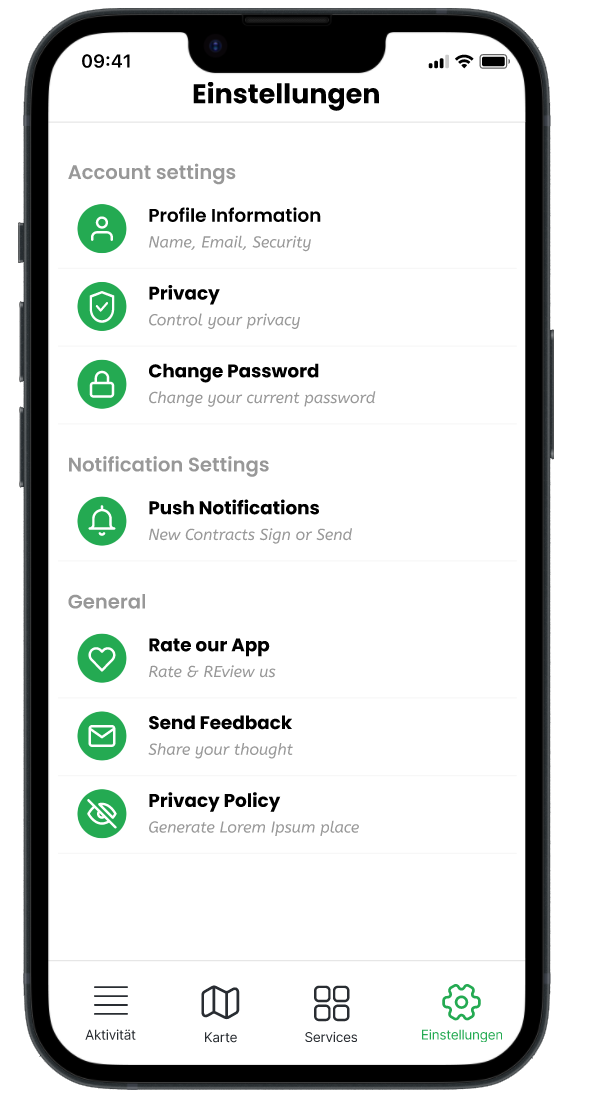
\includegraphics[width=0.3\textwidth]{images/app_mock_settings}
  \caption{\Gls{Mockup} vom Screen Einstellungen}
  \label{fig:screensettingsmock}
\end{figure}

\bigskip


\paragraph{Services}Der \Gls{Tab} „Services“ dient zum Darstellen verschiedener Dienste. Es gibt eine Möglichkeit zum Teilen eines Entsperrungscodes für ein gelagertes Fahrrad und die Eingabe eines solchen Codes. Außerdem werden mehrere externe Dienstleistungsmöglichkeiten zum Beispiel für das Ausleihen eines E-Scooters oder zum Abgeben von Paketen aufgelistet.

\begin{figure}[H]
  \centering
  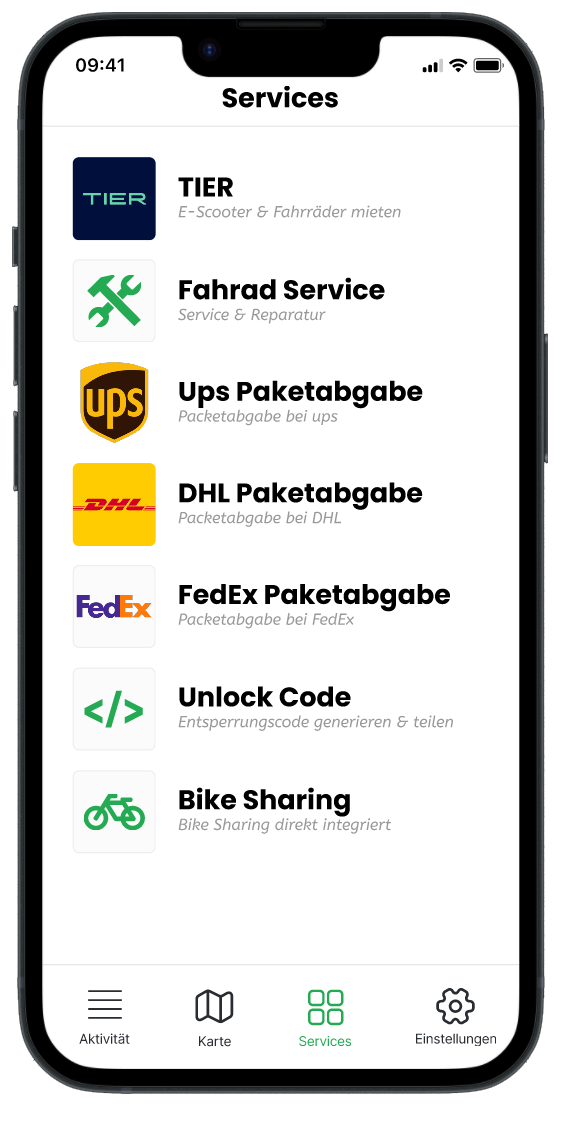
\includegraphics[width=0.3\textwidth]{images/app_mock_services}
  \caption{\Gls{Mockup} vom Screen Services}
  \label{fig:screenservicesmock}
\end{figure}

